\subsection{Basic History}
    In 1959, Moore, Edward F. presented one of the first shortest path through a maze algorithm
    \cite{MooreRef}, after a couple of years in 1961 Lee, C. Y. presented the idea of simulating the 
    board wiring on electronics board as a Maze \cite{LeeRef}. Starting from there the idea of Lee Maze
    has been revisited many times, in 1983 Hightower, D. made more contribution to the idea such that
    using modern computers and virtual memories we can memic the routing problem precisely providing 
    different techniques \cite{HightowerRef}.
\subsection{Router Anatomy}
    The Routing problem has many sections and subsections, in this paper we are mainly concerned with
    Detailed routing. Detailed routing is divided into many subsections, as you can see in fig 
    \ref{fig:routing_anat} and we are exploring Maze and Line Search subsections.

    \begin{figure}[H]
        \centering
        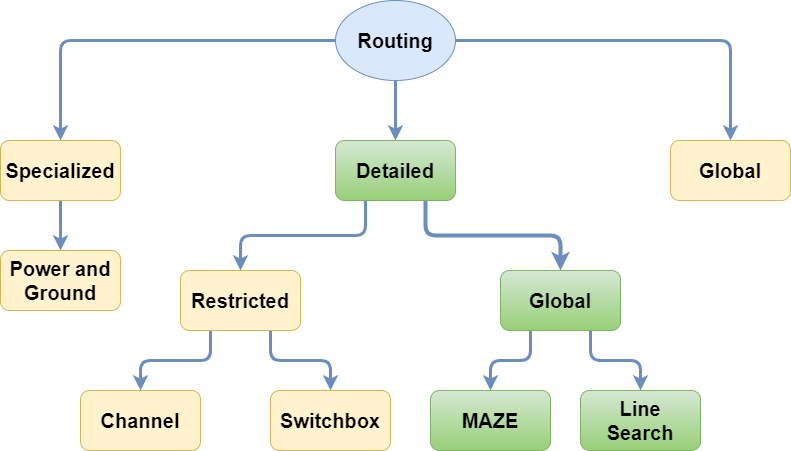
\includegraphics[width=0.4\textwidth]{figures/routing_anatomy.png}
        \caption{Anatomy of various routing techniques.}
        \label{fig:routing_anat}
    \end{figure}

    In the next section we are showing how various algorithms work, and discussing three 
    algorithms, first the \nameref{LeeSection} it's a Maze based algorithm, second the 
    \nameref{MikamiSection} it's a Line-Probe algorithm, and finally the \nameref{SteinerSection} 
    it's a baseline algorithm.

\subsection{Explored Techniques}
    \subsubsection{Lee algorithm}
    \label{LeeSection}
    \subsubsection{Mikami algorithm}
    \label{MikamiSection}
    \subsubsection{Steiner algorithm}
    \label{SteinerSection}
    
